\chapter{Offline Experiment}

\section{Simulated User Queries}
\label{app:user_queries}

\begin{figure}[h]
    \centering
    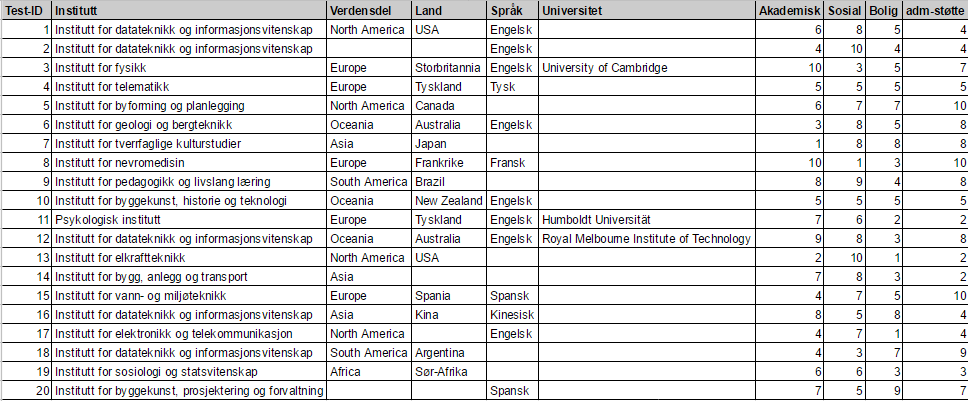
\includegraphics[width=1.0\textwidth]{fig/simulated_queries.PNG}
    \caption[]{20 simulated user queries}
    \label{fig:my_label}
\end{figure}


\section{Results}

\begin{table}[H]
\small
\centering
\caption[]{Full results of the offline experiment}
\label{app:full_offline_test_results}
\begin{tabulary}{\textwidth}{CRR}
\textbf{Query \#} & \textbf{Similarity based retrieval (0-60)} & \textbf{Simulated exact match search (0-60)}\\ \hline
1 & 44.5 & 32.0 \\\hline
2 & 34.5 & 27.0 \\\hline
3 & 36.5 & 28.0 \\\hline
4 & 39.5 & 32.0 \\\hline
5 & 41.0 & 32.5 \\\hline
6 & 39.5 & 34.5 \\\hline
7 & 34.5 & 28.0 \\\hline
8 & 41.0 & 37.5 \\\hline
9 & 33.5 & 29.5 \\\hline
10 & 36.5 & 26.5 \\\hline
11 & 35.0 & 32.5 \\\hline
12 & 39.0 & 34.5 \\\hline
13 & 41.5 & 32.5 \\\hline
14 & 36.5 & 28.5 \\\hline
15 & 39.0 & 26.5 \\\hline
16 & 26.5 & 20.5 \\\hline
17 & 36.5 & 29.5 \\\hline
18 & 34.5 & 31.0 \\\hline
19 & 37.0 & 33.0 \\\hline
20 & 27.5 & 25.0 \\ \hline
\textbf{Mean} & 36.7 & 30.05 \\ \hline
\textbf{STD} & 4.36 & 3.93
\end{tabulary}
\end{table}